\documentclass[__main__.tex]{subfiles}

\begin{document}

\section{Спектральный признак устойчивости схемы Кранка-Николсона для одномерного параболического уравнения}
Cхема Кранка-Николсона: \\
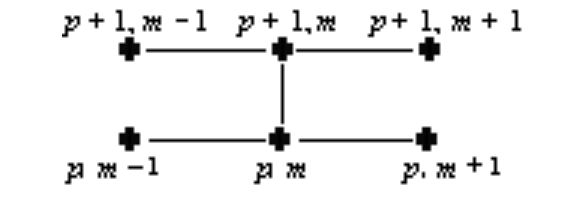
\includegraphics[scale = 0.7]{img_31_1}
$$\frac{U_m^{n+1}-U_{m}^{n}}{\tau} - \frac{a^2}{h^2}[\sigma(U_{m-1}^{n+1}-2U_{m}^{n+1}+U_{m+1}^{n+1}) + (1-\sigma)(U_{m-1}^{n}-2U_m^n+U_{m+1}^{n})] = f_m^{p+1/2}$$
- это общий вид для шеститочечной параметрической схемы. При $\sigma = 1/2$ будет являться схемой Кранка-Николсона. \\
Порядок аппроксимации при $\sigma = 1/2$: $O(\tau^2+h^2)$ \\
Введем обозначения:
$ K = a^2r$,  $r =\frac{\tau}{h^2}$ \\
Тогда для $\sigma = 1/2$ схема устойчива при любых $K$. \\
Следовательно, схема Кранка-Николсона абсолютно устойчива.



\end{document}
